\documentclass[12pt,a4paper]{extarticle}
\usepackage[margin=1.8cm,bottom=2cm]{geometry}
\usepackage{authblk}
\usepackage{float}
\usepackage{pdflscape}
\usepackage{graphicx}
\usepackage{booktabs}
\usepackage[hidelinks]{hyperref}
\usepackage[style=authoryear-icomp,
uniquelist=false,
maxnames=2,
minnames=1,
maxbibnames=99,
    backend=biber, giveninits=true,
    ibidtracker=false,
    uniquename=false,
    natbib=true]{biblatex}

\addbibresource{../battery_paper/DCE_lit_review.bib}
\addbibresource{../battery_paper/Used EV.bib}
\addbibresource{../battery_paper/EV battery.bib}

\AtEveryBibitem{%
  \clearfield{url}%
  \clearfield{urldate}%
  \clearfield{note}%
}

\setlength{\parskip}{2pt}

\renewcommand\Authfont{\fontsize{10}{12}\selectfont}
\renewcommand\Affilfont{\fontsize{10}{12}\selectfont}
\renewcommand\Authand{, }
\renewcommand\Authands{, }

\date{}

\begin{document}

\title{\fontsize{14}{17}\selectfont\textbf{Consumer Preferences in the Used Vehicle Market: Willingness to Pay for Powertrain Type, Driving Range, Vehicle Condition, and Operating Cost}}

\author[1]{Zain Hoda}
\author[1,2]{Xiatian Iogansen}
\author[2]{Christina Gore}
\author[2]{Joshua D. Kneifel}
\author[1,2]{Sindhu Ranganath}
\author[1]{John P. Helveston}

\affil[1]{Department of Engineering Management and Systems Engineering, George Washington University}
\affil[2]{Applied Economics Office, Engineering Laboratory, National Institute of Standards and Technology}

\maketitle
\vspace{0.5em}

\section*{Background}

\section*{Data and Method}

\section*{Results}

\clearpage
\begin{landscape}
\begin{figure}[H]
    \centering
    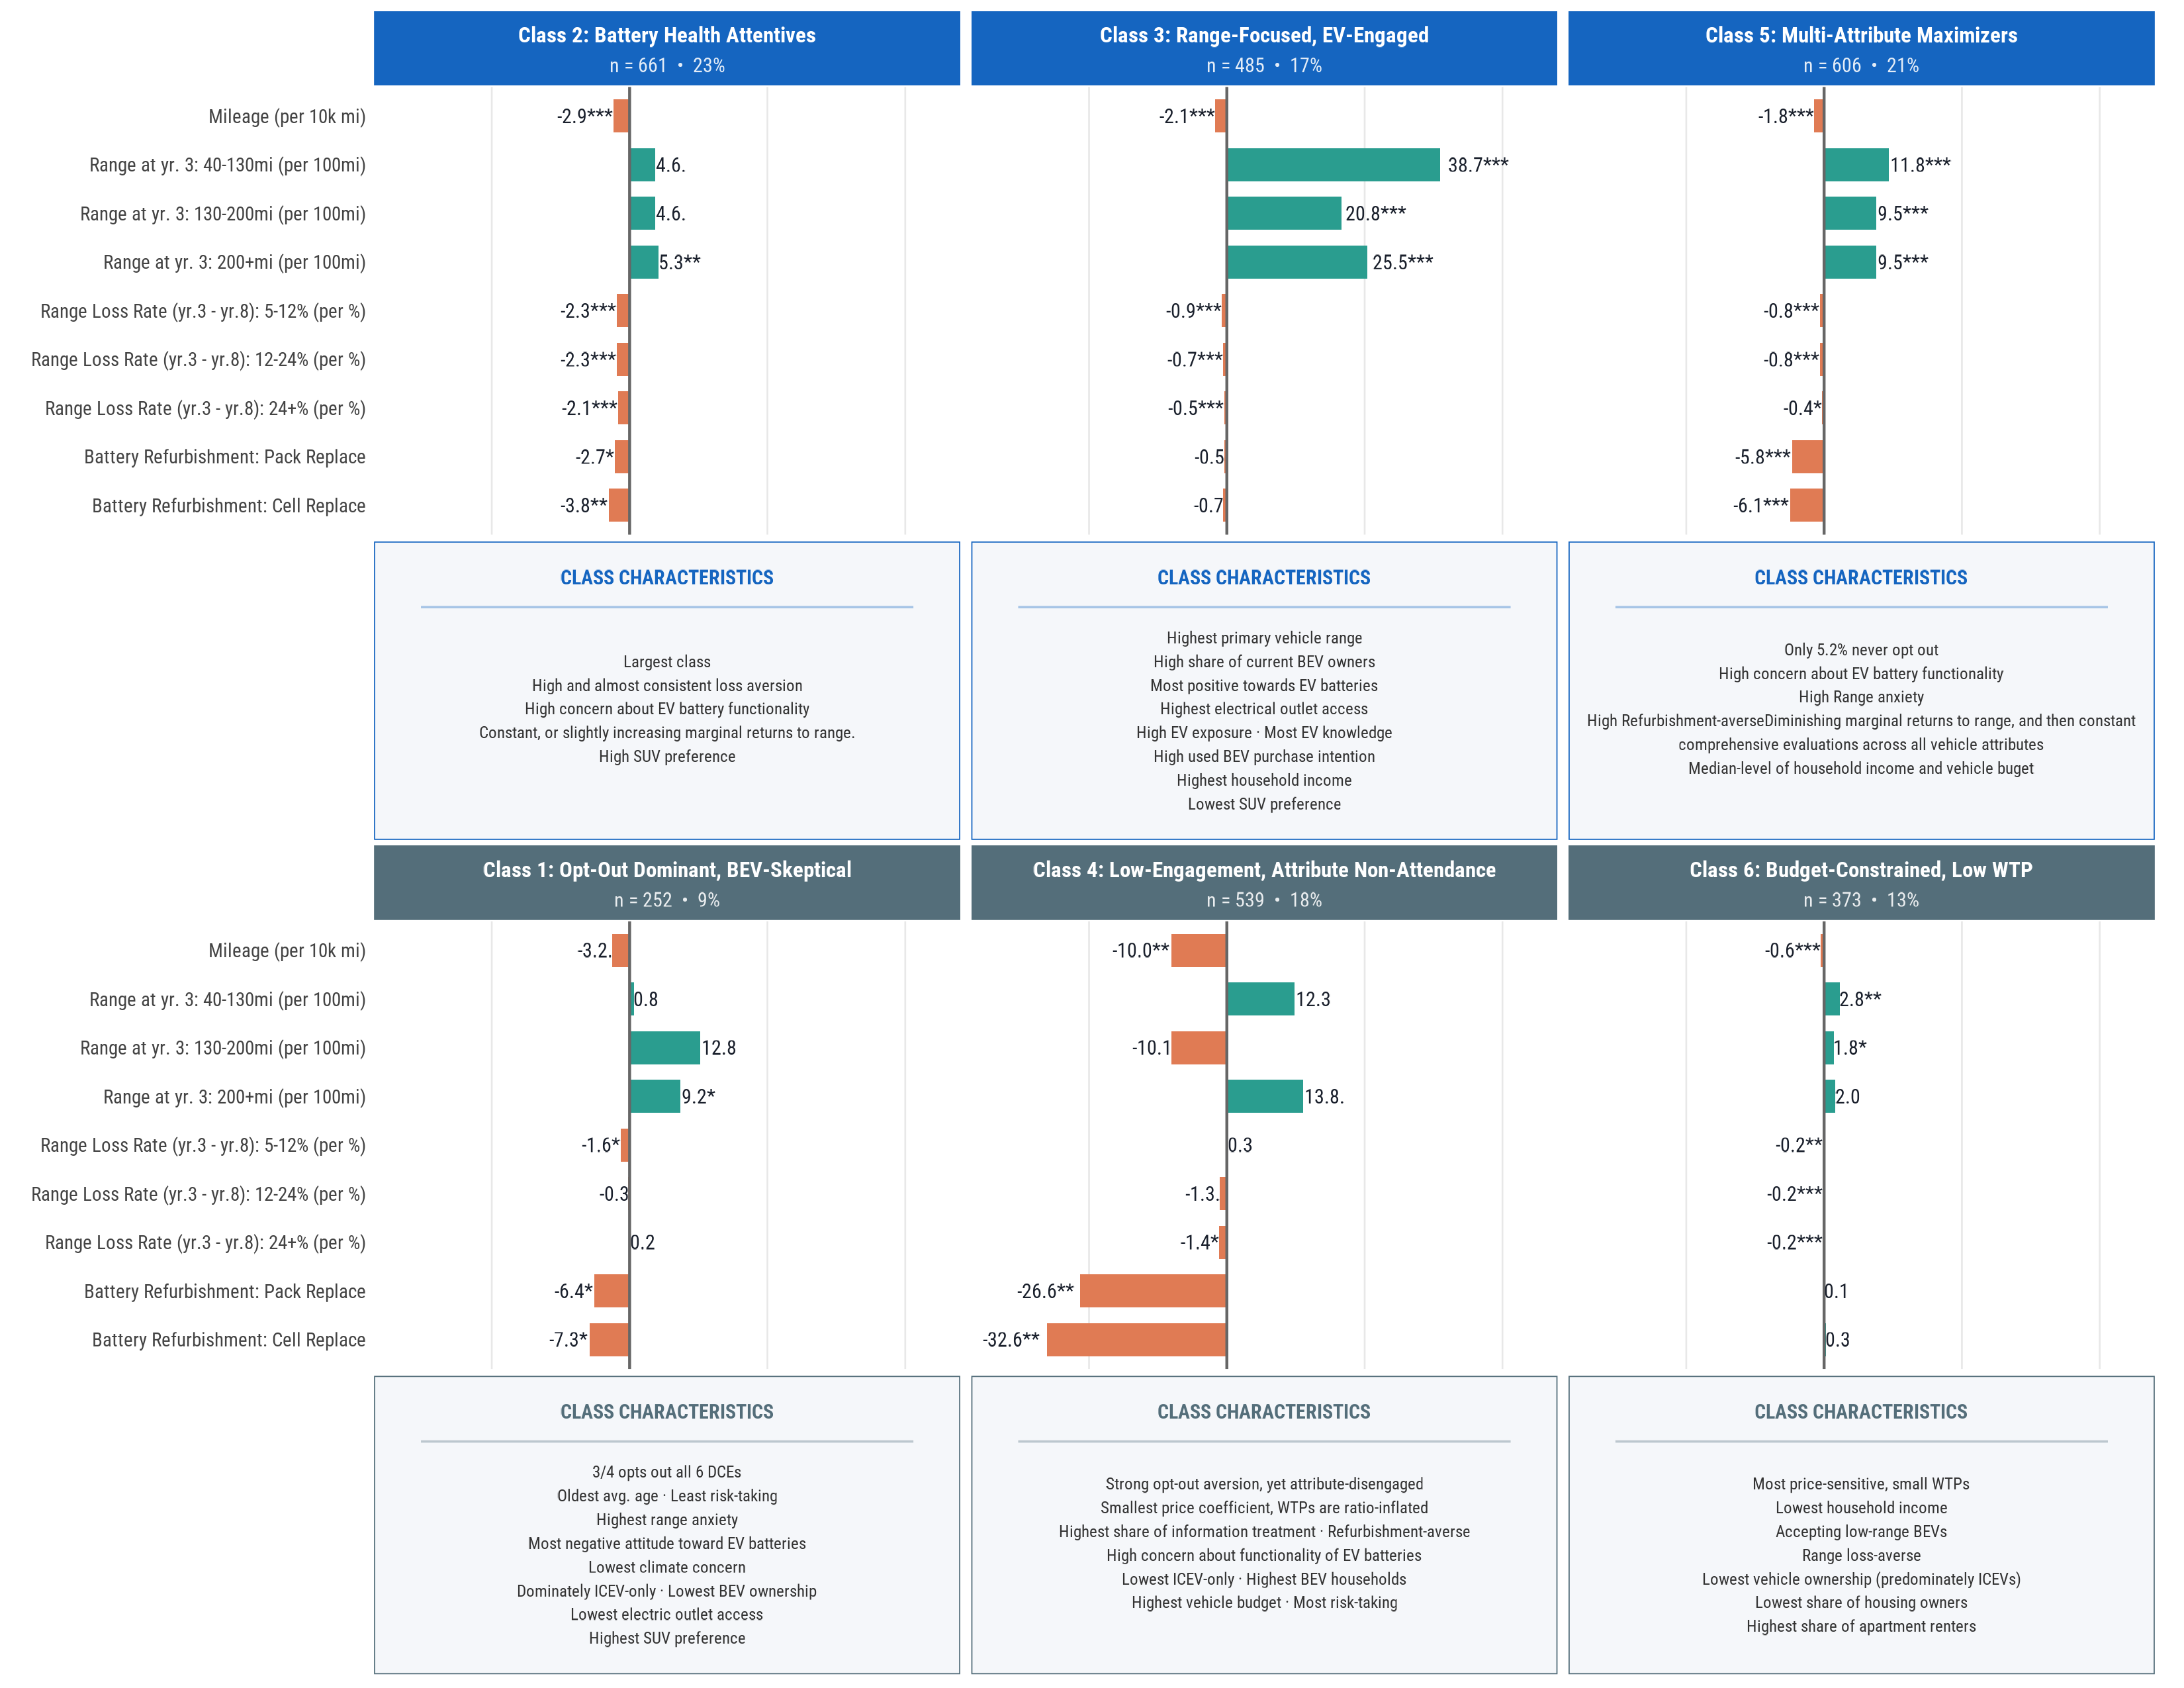
\includegraphics[width=0.94\linewidth, keepaspectratio]{../../code/output/model_output/battery_analysis/apollo/0_lc6_class_profiles_no_optout.png}
    \caption{WTP and class profile summary.}
    \label{fig:lc6_class_profiles}
\end{figure}
\end{landscape}

\clearpage
\begin{center}
{\fontsize{14}{17}\selectfont\textbf{Consumer Valuation of Battery Health Attributes in Used Battery Electric Vehicle Markets: A Discrete Choice Experiment}\par}
\vspace{0.5em}
{\fontsize{10}{12}\selectfont
Xiatian Iogansen\textsuperscript{1,2},
Zain Hoda\textsuperscript{1},
Christina Gore\textsuperscript{2},
Joshua D. Kneifel\textsuperscript{2},
Sindhu Ranganath\textsuperscript{1,2},
John P. Helveston\textsuperscript{1}\par}
\vspace{0.3em}
{\fontsize{10}{12}\selectfont
\textsuperscript{1}Department of Engineering Management and Systems Engineering, George Washington University\par
\textsuperscript{2}Applied Economics Office, Engineering Laboratory, National Institute of Standards and Technology\par}
\end{center}
\vspace{-1.5em}

\section*{Background}

Used vehicle transactions account for roughly 70\% of U.S. passenger vehicle purchases, and used BEVs are entering the secondary market at an accelerating pace \parencite{coxautomotiveinc.EVMarketMonitor2025}. Despite this, 52\% of U.S. adults are unlikely to consider a used BEV purchase \parencite{fernandesUSUnderstandingConsumer2023}, primarily citing uncertainty about battery condition. This information gap suppresses demand and prevents efficient pricing in the secondary market.

\section*{Data and Method}

We administered an online discrete choice experiment (December 2025--April 2026) to 3,072 U.S. adults intending to purchase a used car or SUV within two years. Each respondent completed six repeated choice tasks selecting among three hypothetical used BEVs or a no-choice option, with attributes varying on mileage, purchase price, electric range at Year~3, annual battery degradation rate, and battery refurbishment history. The design was stratified by body type (car or SUV) and budget ($\leq$\$20,000 vs.\ $>$\$20,000), and half the sample received extended battery cost and warranty information to test whether additional detail changes choices.

We estimate a six-class Latent Class Choice Model (LCCM) on 2,916 respondents with complete covariate data (17,496 choice observations). The LCCM consists of a class membership model (which assigns respondents probabilistically to classes based on attitudes, infrastructure access, and demographics) and a class-specific choice model (which estimates conditional choice probabilities within each class). Class-specific WTP is the negative ratio of the attribute coefficient to the price coefficient. The paragraphs below summarize the WTP characteristics and segment profiles of each class. Figure~\ref{fig:lc6_class_profiles} provides a visual overview of all six segments.

\section*{Results}

\textbf{Class 1: Battery Health Attentives ($n$=661, 22.7\%).} Range loss aversion is the highest across all classes, at approximately \$2,300*** per percentage point across all three degradation segments. Both refurbishment types generate meaningful disutility (pack: -\$2,740*, cell: -\$3,760**). Range WTP is consistent across piecewise segments (\$4,570, \$4,610, \$5,310**). Members are well-informed (BEV knowledge: 76.2\%) and are effectively purchasing battery reliability rather than range.

\textbf{Class 2: Multi-Attribute Maximizers ($n$=606, 20.8\%).} This class places the highest premium on crossing the minimum viable range threshold (\$11,830***), with uniform range loss aversion (-\$780*** to -\$390*) and the highest refurbishment disutility among attribute-sensitive classes (pack: -\$5,760***, cell: -\$6,070***). Only 5.2\% never opt out; respondents opt out when no option meets their quality standard across all dimensions.

\textbf{Class 3: Range-Focused, EV-Knowledgeable Consumers ($n$=485, 16.6\%).} WTP for range is exceptionally high below 130 miles (\$38,700*** per 100 miles), declining sharply thereafter (\$20,820***), with uniformly significant range loss aversion (-\$870*** to -\$470***). WTP for refurbishment is negligible. Members are the most BEV-knowledgeable (81.1\%), highest-income (\$97,120), and most favorable toward refurbished batteries.

\textbf{Class 4: Budget-constrained, Low-WTP Consumers ($n$=373, 12.8\%).} The largest price coefficient in absolute value (-4.017***) identifies these buyers as budget-constrained. Range WTPs are modest (\$2,810** and \$1,800*) and refurbishment penalties are negligible. Despite strong price sensitivity, 91.2\% never opt out. Members have the lowest income (\$70,000), lowest homeownership rate (43.0\%), and highest renter share (48.8\%).

\textbf{Class 5: Opt-Out Dominant, BEV-Skeptical Consumers ($n$=252, 8.7\%).} Systematic opt-out defines this class (75.4\% chose no-vehicle in all six tasks), with most attribute WTPs indistinguishable from zero. Significant penalties exist only for range loss (-\$1,620*) and refurbishment (pack: -\$6,350*, cell: -\$7,320*). Members are the oldest (47.1 years), least risk-tolerant (24.0\%), and have the highest range anxiety (87.2\%).

\textbf{Class 6: Low-Engagement, Attribute Non-Attendance Respondents ($n$=539, 18.5\%).} The near-zero price coefficient (-0.144**) mechanically inflates all WTP ratios. The pattern is consistent with attribute non-attendance: mileage carries a large, isolated valuation (-\$9,950**) while most other attributes are imprecisely estimated. WTP estimates for this class are treated as unreliable.

This paper delivers the first WTP estimates for battery health attributes in the U.S. used BEV market from a national DCE of 3,072 respondents. Consumers fall into six segments that differ markedly in battery quality sensitivity, price responsiveness, and market engagement. Classes~1 and~2 (43.5\% combined) prioritize battery health and are the primary market for certified battery-health disclosure. Class~3 (16.6\%) is BEV-engaged but responds to range, not refurbishment history. Class~4 (12.8\%) is price-constrained and largely indifferent to battery quality signals, while Class~5 (8.7\%) represents consumers not yet viable in the used BEV market.

For dealers and OEMs, these results support standardized battery health certification: independent verification of state of health, degradation history, and remaining warranty coverage could command measurable price premiums from the quality-sensitive majority. Cell and pack replacement are penalized at similar magnitudes despite their technical differences, pointing to a market opportunity for certification services that distinguish high-quality refurbishment from simple repair and communicate it in terms consumers understand.


\begingroup
\setlength{\bibitemsep}{0pt}
\setlength{\bibnamesep}{0pt}
\renewcommand{\bibfont}{\scriptsize}
\printbibliography[heading=none]
\endgroup

\clearpage
\begin{landscape}
\begin{figure}[H]
    \centering
    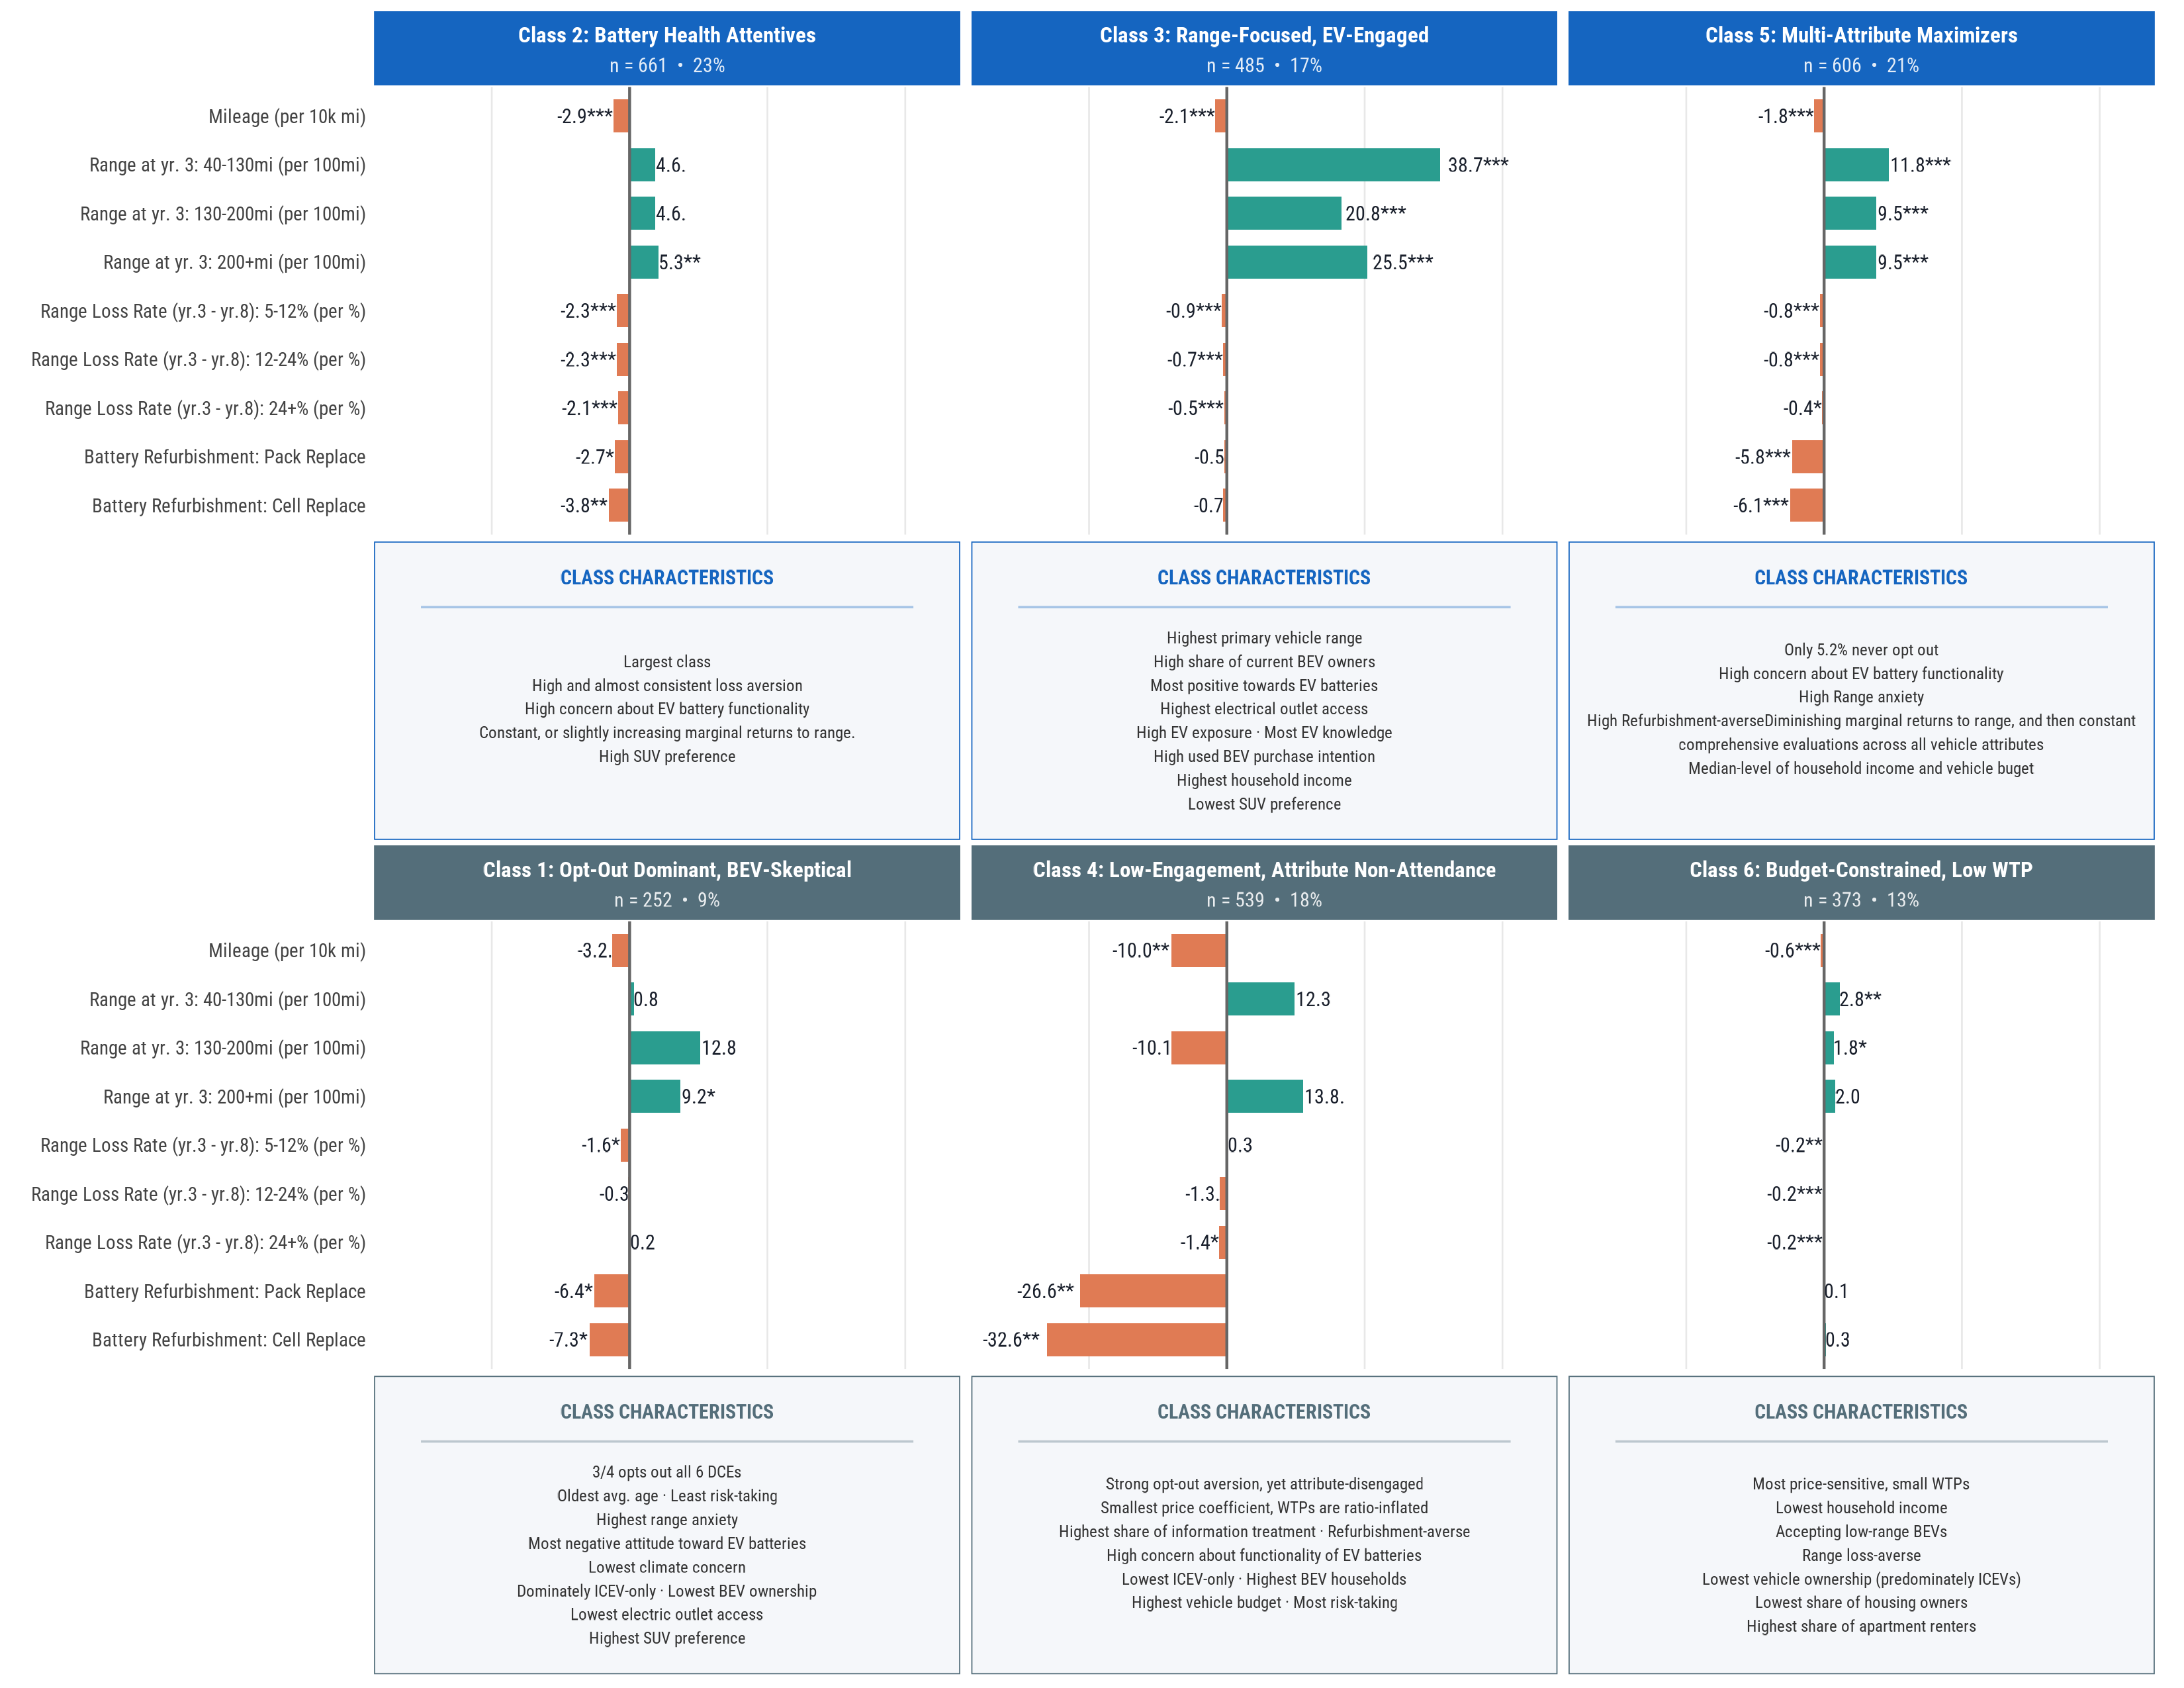
\includegraphics[width=0.94\linewidth, keepaspectratio]{../../code/output/model_output/battery_analysis/apollo/0_lc6_class_profiles_no_optout.png}
    \caption{WTP and class profile summary.}
    \label{fig:lc6_class_profiles}
\end{figure}
\end{landscape}

\end{document}
